% !BIB TS-program = biber
%--------------------
% Packages
% -------------------
\documentclass[11pt,a4paper]{article}

\usepackage{mathptmx} % Use Times Font
\usepackage{times}
\usepackage{amsmath}
\usepackage[style=authoryear,backend=biber]{biblatex} %Imports biblatex package
\addbibresource{ed_extra.bib} %Import the bibliography file
\addbibresource{database.bib}
\usepackage[pdftex]{graphicx} % Required for including pictures

\usepackage[pdftex,linkcolor=black,pdfborder={0 0 0}]{hyperref} % Format links for pdf
\usepackage{calc} % To reset the counter in the document after title page
\usepackage{enumitem} % Includes lists

\frenchspacing % No double spacing between sentences
\linespread{1.2} % Set linespace
\usepackage[a4paper, lmargin=0.1666\paperwidth, rmargin=0.1666\paperwidth, tmargin=0.1111\paperheight, bmargin=0.1111\paperheight]{geometry} %margins
%\usepackage{parskip}

\usepackage[all]{nowidow} % Tries to remove widows
\usepackage[protrusion=true,expansion=true]{microtype} % Improves typography, load after fontpackage is selected




%-----------------------
% Set pdf information and add title, fill in the fields
%-----------------------
\hypersetup{ 	
pdfsubject = {},
pdftitle = {},
pdfauthor = {}
}
\title{Attribution of the  extreme precipitation related to the August 12th 2020 Carmont, Scotland derailment.}
\author{Simon Tett, School of Geosciences, University of Edinburgh}

%-----------------------
% Begin document
%-----------------------
\begin{document}
\maketitle
\graphicspath{{../figures/}}
\begin{abstract}
	The UK's Convective Permitting Model suggests, in the Stonehaven area, that extreme hourly rainfall changes at Clausius–Clapton +50\%. This leads to an increased probability, relative to late 19th century conditions,  of rainfall similar to the rain that was associated with the fatal rail accident in Carmont on August 12th 2020, by about 30\% with a doubling of probability for such events in a +2K warmer world. Some characteristics of the simulated extreme rain evaluate well against radar values but the  simulated rainfall is about 20-30\% larger than the radar rainfall. This may reflect model problems or shortcomings in  radar  calibration. 
\end{abstract}

\section{Introduction}

On August 12th 2020 a passenger train running from Aberdeen to Glasgow derailed at Carmont near Stonehaven. The train was lightly loaded due to COVID restrictions but three people died and the remaining six people on the train  were injured. The proximate cause of the derailment was gravel being washed out of a drain \parencite{carmontReport2024}. Radar estimates of  rain at 1km x 1km resolution was 51.5 mm of rain falling between 05:50 to 09:00 which was estimated at around a 1-in-a-100 year event. The drain should have been able to deal with that volume of water but because the drain had not been built to design requirements gravel and other debris was washed out of it and onto the tracks. 

Given the small size of the drainage area, then how climate change might have changed the risk of hourly extreme rainfall is a relevant scientific question. My goal was to apply a similar methodology to that of  \textcite{Tett2023} which used a combination of radar rainfall and simulated data from the Convective Permitting Models (CPMs) ran for the UKCP18 project\parencite{ukcp2019cpm} to estimate return periods and change in return period. The aim of my work at the Met Office was to work with colleagues there, refine my definition of events and carry out some evaluation of the CPM ensemble through comparison of it with radar data. While I was visiting the Met Office a bug with the simulations had been discovered and an empirical technique to filter out the impact of that error been developed. Part of this report will examine the effect of filtering on the response of extreme precipitation to warming. 

Theory\parencite{allen02insight} suggests that extreme rainfall occurs when the entire column of atmospheric water precipitates. This, in turn,  suggests that extreme precipitation increases fractionally at the same rate as saturated humidity, or for fixed atmospheric pressure, saturated vapour pressure. This is about 7\%/K. However, some studies suggest that sub-daily extreme rainfall  will increase  ar rates faster than this. 



\section{Methods}
In this section I describe the methods used in the analysis. They are split into processing of the Convective Permitting Model to remove unphysical rain events  and computation of maxima, how the radar is analysed, definition of an event and, finally, how probabilities of exceeding thresholds are computed. 

All analysis uses a 150x150 km square region with Stonehaven in the centre. In order to avoid topographic effects and work with a homogenious region only land cells with a height of 300m or less were included in the analysis. As the derailment happened in August analysis is restricted to June-July-August. 

\subsection{CPM data processing}

Due to a bug in the model dynamics code the UKCP18 convective permitting models generate unphysical rainfall when the data is advected along grid lines. Software was developed by Simon Brown to empirically filter out such lines of extreme rain and the occasional point with extreme rainfall by processing the hourly precipitation model output. This software has several empirical constants to select thresholds and sizes. The default values were used.  

Both the filtered ("Filt CPM") and raw ("Raw CPM") data were then aggregated to 4.4 km resolution by simple averaging over 4 cells. Then, for each grid point, I computed the seasonal hourly maximum and date/time of maxima for all seasons and  years in the ensemble. 

\subsection{Radar analysis}
Radar data is available in daily files with  1km 5-minute and 5km 15-minute available.  Both datasets  were aggregated to hourly means requiring, for any day, data from at least 6  unique hours. As a crude form of quality control data was set missing if the rain rate was greater than 400 mm/hour.  The 1km data was then aggregated to 4 and 5km resolution by averaging 16 or 25 cells respectively. The daily maximum and time of maximum were computed and then the seasonal maxima and maxima time/date calculated. This gives three radar datasets (radar 5km, radar 1kmc4 and radar 1kmc5). I use these radar datasets to give a qualitative uncertainty estimate.

Radar datasets can suffer from various artefacts \parencite{artefacts}.
For the Stonehaven region, both the mean summer rainfall and the summer mean 1-hour maximum rainfall are largely free of artefacts (Fig~\ref{fig:mean_rain}). There are two artefacts associated with the Munduff hill site on the southern end of the domain visible in the summer mean rain. Beyond these the clearest signal is a strong land/sea contrast in both the mean and maximum rain. 

\subsection{Event Definition}

One goal of the study was to use the large volumes of radar data to compare with data from the CPM stimulations. I  wanted  to fit distributions to  datasets of seasonal extreme rainfall and compare the distributional properties. To properly estimate uncertainties requires a dataset of independent values but extreme rainfall in two locations close in space and time is likely from the same system and so not independent. Solving this  well is applied statistics, and well beyond the scope of this project, so I have chosen a crude way of doing it.  An event is defined as all extreme rainfall occurring on the same day where the surface height is between 0 and 300m. 300m is below the level of the highest topography in the region. Within that event quantiles are computed at values from $0$ to $1$ in steps of $0.05$. Each of these quantile values have their position, time, and topographic height recorded. The event area is also recorded. 

Figure~\ref{fig:example_event} shows maximum hourly precipitation for summer 2020 and  extreme precipitation for the August 12th event. The August 12th event had an area of about 4000 km$^2$ which makes it a rare event. 


\subsection{Statistical Models}

I fit several different statistical models to the simulated  extreme event data. Each event quantile has a  statistical model fit independent of any other quantile value and I use the Akaike Information Criteria (AIC) to decide on the best model\parencite{akaike74aic}. These models were fit using the extRemes R library\parencite{gilleland2016extremes} giving, with uncertainties, the parameters for a Generalised Extreme Value (GEV) distribution.   This library allows covariates to be included in the fit. I assumed a fixed shape with the location and scale parameters changing linearly with covariates selected from  Central England Temperature (CET), CET$^2$,  $\log_{10}$ of the event area, and the event area.  Use of CET was based on my earlier work\parencite{Tett2023} and, for the ensemble, CET correlates well with regional saturated vapour pressure~(Fig.~\ref{fig:cet_scatter}). 

 
 Use of CET$^2$ allows non-linear impacts to be examined while use of  event area or $\log_{10}$ event area is plausible as one would expect the large quantiles to be larger for big events - though how much depends on the correlation scale between extreme rainfall within an event. 

Adding covariates does reduces the AIC across all quantiles suggesting an improvement over no covariate(Figure~\ref{fig:aic}). The minimum AIC, at all quantiles, is when CET, CET$^2$,  and $\log_{10}$ area are used. However at the larger quantiles including area or $\log_{10}$ area causes a larger reduction in AIC than does CET.  Most improvement come from use of CET and $\log_{10}$ area suggesting that non-linear effects are small and I use those two covariates from here on. 
The simulated CET records show a range of different behaviours and biases (Fig.~\ref{fig:summer_cet}). So, use of CET covariate also corrects for biases in the model simulations. 


\section{Results}

Table~\ref{tab:summary} summarizes various properties of the radar and CPM events for the Stonehaven region.  Both the number of events and the median event area are broadly comparable though the model has more events/year than the radar does.  However, the CPM has about 30\% too much extreme rain in the median quantile of events even after filtering precipitation. Examining  all seasonal extremes in the region the filtered model has about 25\% more rain than the radar data.  This might be because of problems in the model or in the calibration of the radar data. 

To see how good the CPM is I compare the distributions of  day-hour, height and  $\log_{10}$ area of the event between the two sets of simulated data and the three radar datasets. For the hour and height I selected the 50\% quantile within the events. Though there are differences between model and radar datasets in broad terms model and radar agree. The main differences are that the simulated day-of-hour has smallest density around 06:00 while the radar data has a fairly flat probability during the late night/early morning. Filtering makes little difference to the day-hour and height distributions -- recall that each quantile has an associated position, height and date/time. Filtering reduces the frequency of about 20 km$^2$ (2x2 grid points) events but still above the density of 16 km$^2$ events (4x4 radar grid points). 

Examining all events from the filtered and raw CPM simulations suggests no relationship between CET and day-hour, height and $\log_{10}$ area in either the raw or filtered data (Fig~\ref{fig:cet_covar}). This justifies not using those variables as covariates in the statistical modelling. 

I focus on the following  model for the location ($\mu$), scale $\sigma$ and shape ($\zeta$) parameters :
\begin{align}
	\mu(C,A) =& \mu_0 + C\mu_\text{CET}+A\mu_{\log_{10}A} \\
	 \sigma(C,A) =& \sigma_0 +C\sigma_\text{CET}+A\sigma_{\log_{10}A}\\
	 \zeta(C,A)=&\zeta_0
\end{align}

Where $C$ is the Central England Temperature (CET) and $A$ is the area in km$^2$ of the event.  I then investigate these distributions as a function of quantile within the events.  The scale and location parameters from all three radar dataset are considerably smaller than the parameters for either the raw or filtered CPM data. Uncertainty in the radar data is considerable (Fig~\ref{fig:scale_locn}(a)) but not large enough to make it consistent with either simulated dataset.  Looking at the intensity of one-in-ten-summer events (Fig~\ref{fig:scale_locn}(b)) we can see that simulated intensities are larger for all event quantiles with a small reduction when using the filtered data compared to the raw simualted data. Uncertainties in the radar data are not  negligible either. 

In both model datasets the scale parameter increases faster than CC (Fig~\ref{fig:scale_locn}(c)). The impact of filtering is to increase the change in the scale parameter leading to super-CC behaviour for quantiles from about 50\% to 90\%.  In both datasets there is a sensitivity to event quantile. In the raw data the increase is largest in the central quantiles while in the filtered data the increase is largest at around the 80\% quantile which is suggestive of intensification within the events. 

I now examine the shape parameter, as a function of quantile which  has no covariates.  There is little sensitivity to quantile in any of the datasets though with a weak tendency to larger values at higher quantiles (Fig~\ref{fig:shape_plot}).  Uncertainties in the radar datasets are large both due to sampling and due to differences in processing. In contrast, uncertainty in the CPM estimates are very small. Filtering the CPM data makes the shape parameter somewhat more positive with the differences statistically significant. In broad terms the CPM has small negative  shape parameters so consistent with Gumbal or Weiball distributions while the radar has a positive shape (so unbounded extreme rainfall)  or a Frechet distribution. 

Computing the changing risk is complex as it will require integrating over event size and quantile. So, I leave that for future work  and instead do the  calculation by using the  filtered CPM data and fitting, at each point, a CET covariate dependant GEV distribution.  Using the co-variate dependant GEV allows computation of changes in intensity and probability, at different CET values as a function of return period and  rainfall amount respectively. For the 2012-2021 JJA period intensity changes and probability ratios are quite noisy (Fig~\ref{fig:map_intensity}) with higher ground -- the eastern Garampian mountains  -- showing larger increases in intensity and probability ratios. While over the North Sea changes appear smaller. Clausius-Clapyron driven intensity changes would be around 6\% for 2012-2021 JJA. Almost all of the domain shows changes larger than 6\% suggesting super-Clausius-Clapyron changes in the simulations. 

Extracting data for the Carmont cell (Fig~\ref{fig:int_pr}) shows that intensity changes and probability ratios (PRs) are fairly small in the 1980s. For 2012-2021 intensity changes across much of the distribution are 7\% or so -- about 50\% larger than expected from Clausius-Clapyron. In the +2K world intensity changes reach +14\% (Fig.~\ref{fig:int_pr}(a)). Probability ratios show an increase with Rx1h 
doubling for Rx1h of 30mm (or larger) in the +2K world. In the current world they are vary between a  20 to 40\% increse while in the 1980s probability ratios increase by only a few percent.  However, comparing those to the region used to define events suggests that the Carmont cell is on the low end of the distribution. This is likely a result of noisy fits and reinforces the need to pool space \& time to produce more accurate results. 



\section{Summary and Next Steps}
The convective permitting model, filtered or raw, evaluates remarkably well against radar observations for hour of maximum event, height of event and,except close to the grid scale, event size. However the CPM extreme rainfall is too intense compared to radar in the Stonehaven region. This might be due to problems with the radar data or model problems.  Filtering slightly reduces this discrepency. 

The simulated extreme rainfall shows super-CC behaviour  which varies across the quantiles within the events and is somewhat sensitive to filtering out "fountains". In the filtered data fractional changes in intensity peak at around the 75\% quantile suggesting intensification within events but not at the most extreme values. The sensitivity of intensity changes to filtering suggests the need to explore sensitivity to the empirical parameters used in the filtering.
 
 
 To actually  compute change in risk for an extreme I would need to integrate over event size and event quantile. Doing this will require careful thought and the complexity of the statistical model  that needs to be generated may make doing this very uncertain removing the advantage of trading space to time.  My current thinking is that the most difficult part of the computation is estimating the distribution of maximum rainfall in the radar dataset. I think the best way to do that is to take random samples from radar events across the whole domain. Then fit distributions to that data.  I will pool together changes from the CPM near Carmont, assume they are independent, and use the GEV fit  uncertainties to estimate a final uncertainty. 

 
Rather than computing saturated humidity from the monthly mean time series I will compute it from daily grid point data. Then, I will compare the seasonal/regional average with the CET timeseries.  I also want to see how lower tropospheric  winds change during extreme events. This will also me to see if reductions changes in storm translation speed can explain the changes in extreme intensity. 

\printbibliography %Prints bibliography

\subsection{Acknowledgments}
I am grateful to the Met Office for funding accommodation and subsistence costs for my two week visit to the Met Office (on which much of the work that forms this report was done.) I would also like to thank Fraser Lott for looking after me and lots of useful discussions as well as Simon Brown, Elizabeth Kendon and Chris Short for  taking the time to discuss the convection permitting model with me.

\begin{table}
	\begin{tabular}{ccccc}
		%%Raw CPM: 8.7 mm/h Filt. CPM: 8.4 mm/h radar_5km: 6.8 mm/h radar_1km_c5: 6.5 mm/h radar_1km_c4: 6.6 mm/h
		& & Median & Median & Median\\
		Source & Events/year & event area(km$^2$) & 50\% quantile event (mm/hr) & all data (mm/h)\\
		radar 5km & 23 & 125 & 7.0 & 6.8 \\
		radar 1km\_c5 & 21 & 125 & 6.8 & 6.5\\
		radar 1km\_c4 & 24 & 128 & 6.8 & 6.6\\ \hline
		Raw CPM & 27 & 130  & 9.5 & 8.7\\
		Filt CPM & 28 & 136 & 9.2 & 8.4\\
		
	\end{tabular}
	\label{tab:summary}
	\caption{Summary event statistics for radar and CPM events. }
\end{table}

\begin{figure}
	\centering
	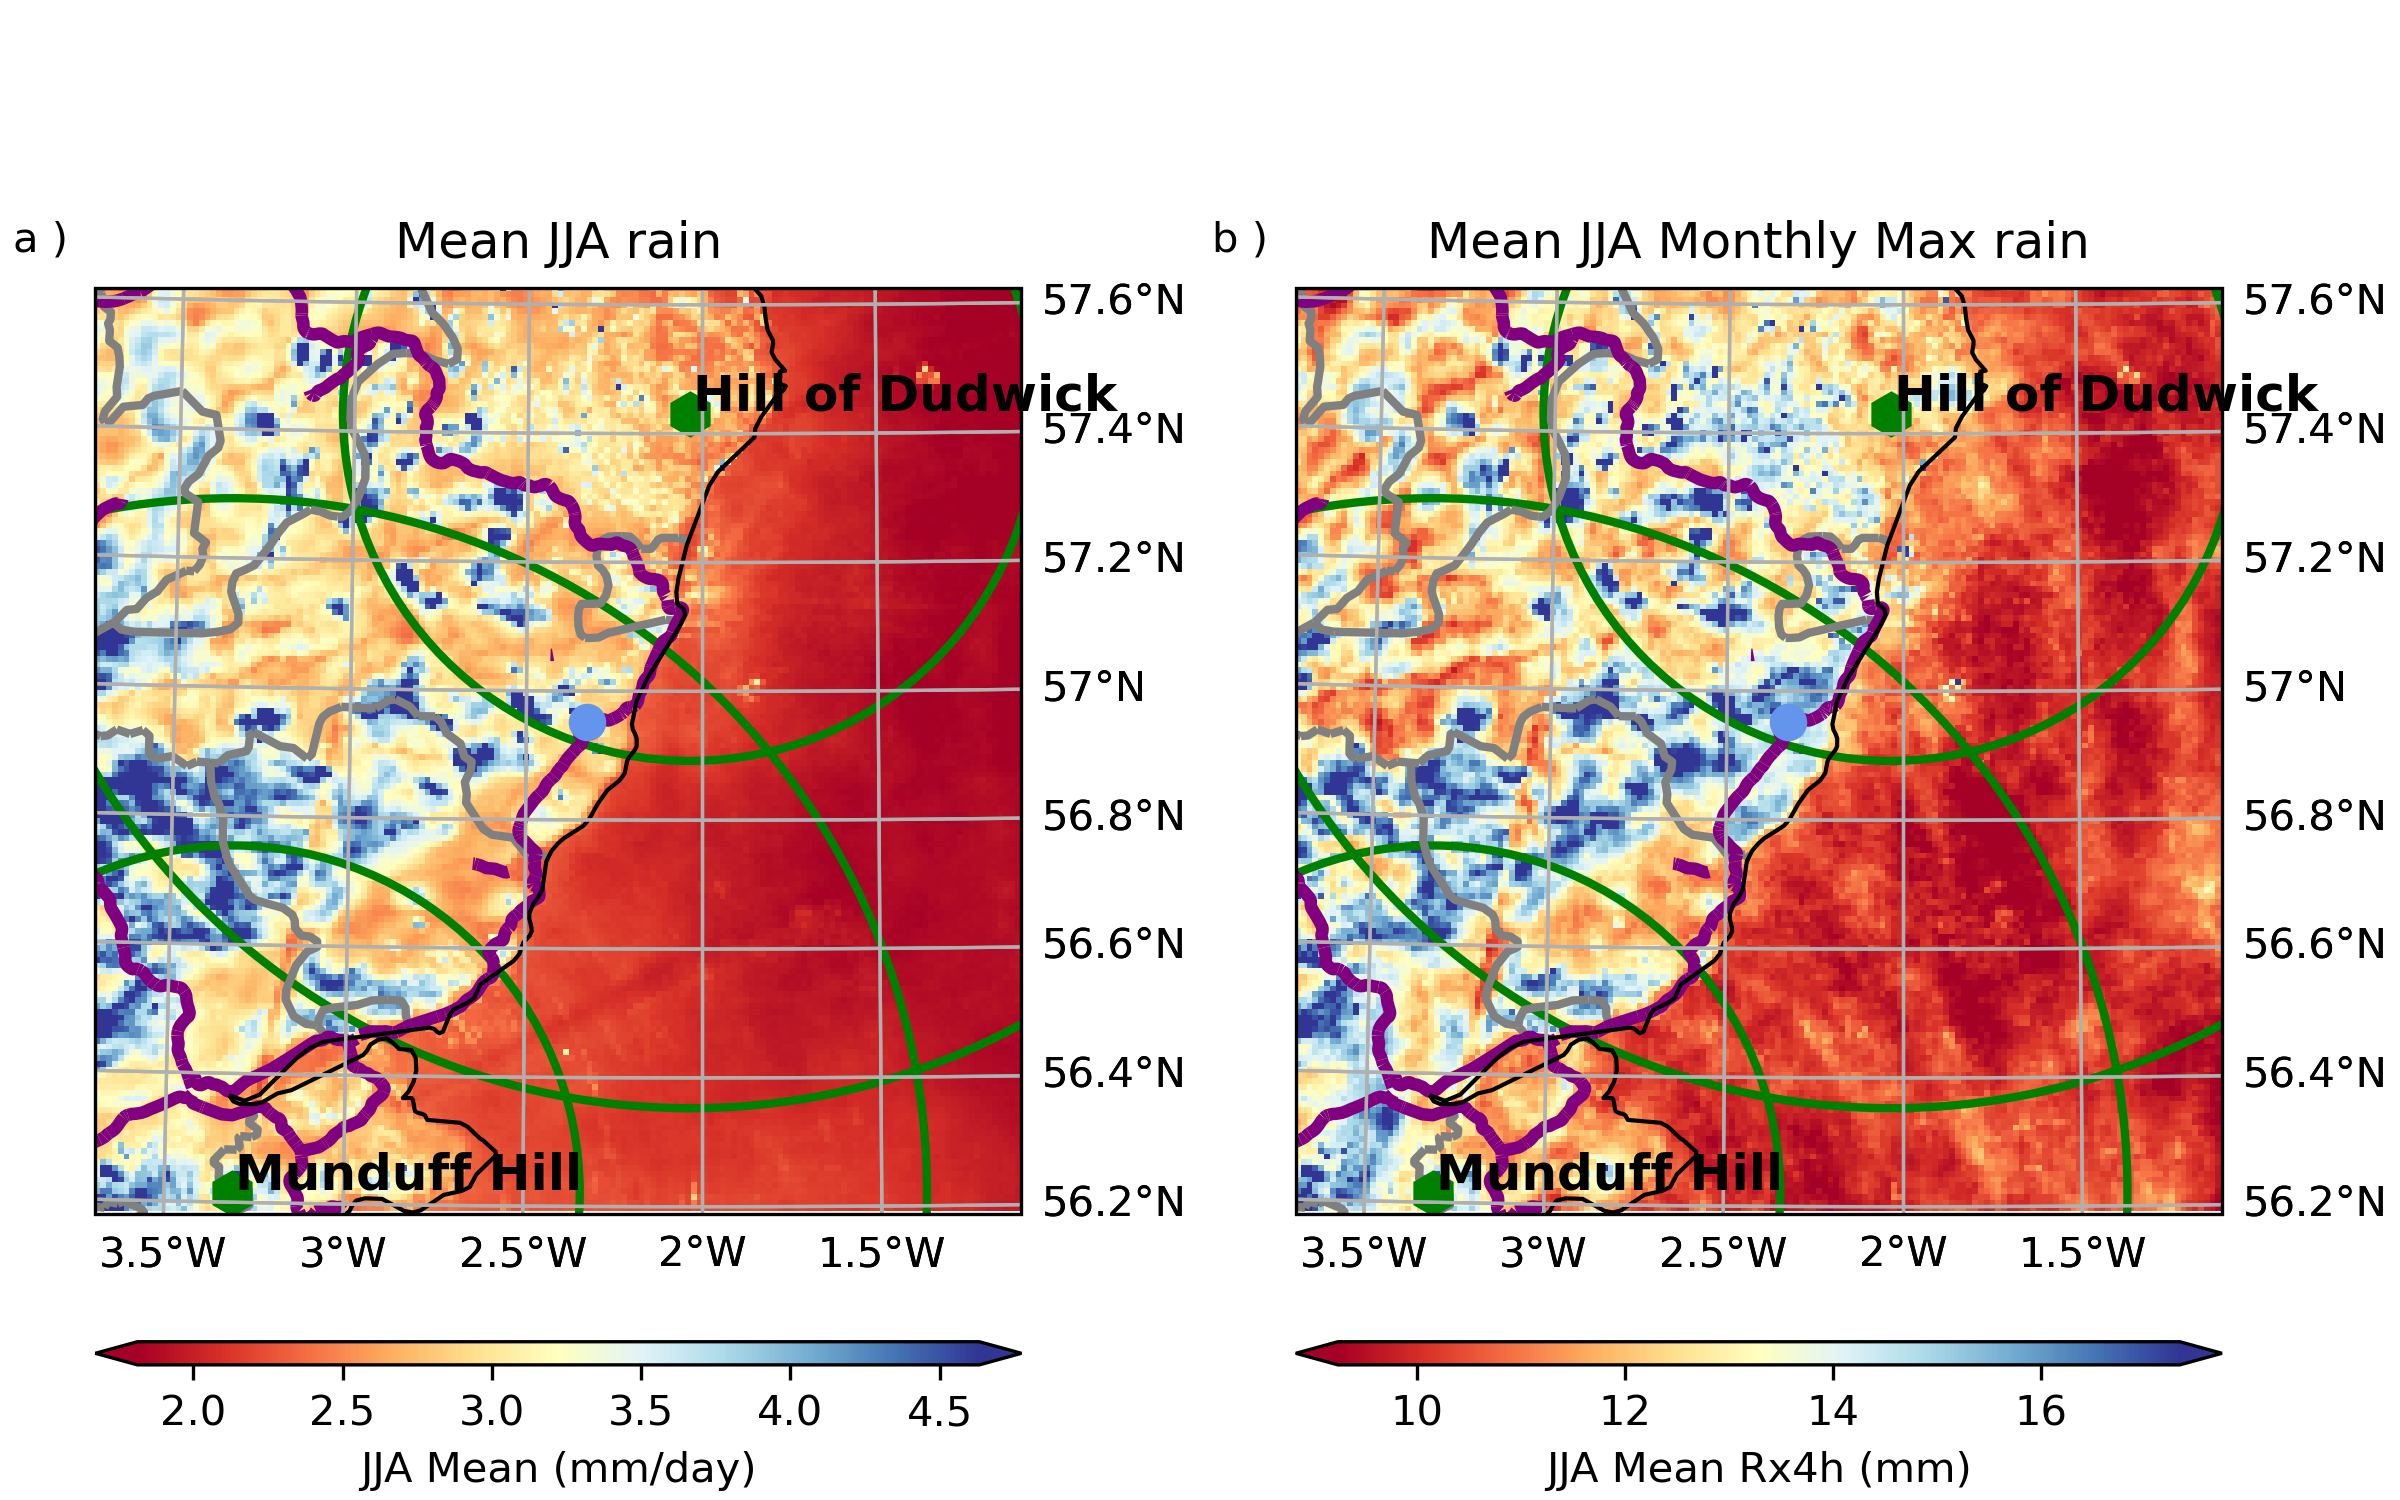
\includegraphics[width=\linewidth]{radar_jja}
	\caption{a) Mean radar rainfall (mm/day) b) Mean monthly maximum 4h rain total (mm/h). Means are for summers (June-July-August) from 2008 to 2023 inclusive. Circles are  60 and 120 km from radar stations (Green hexagons). Pale blue circle shows point ("Carmont drain") where rain occurred, purple lines show railways and grey lines local authority boundaries. }
\end{figure}
\begin{figure}[tp]
	\centering
	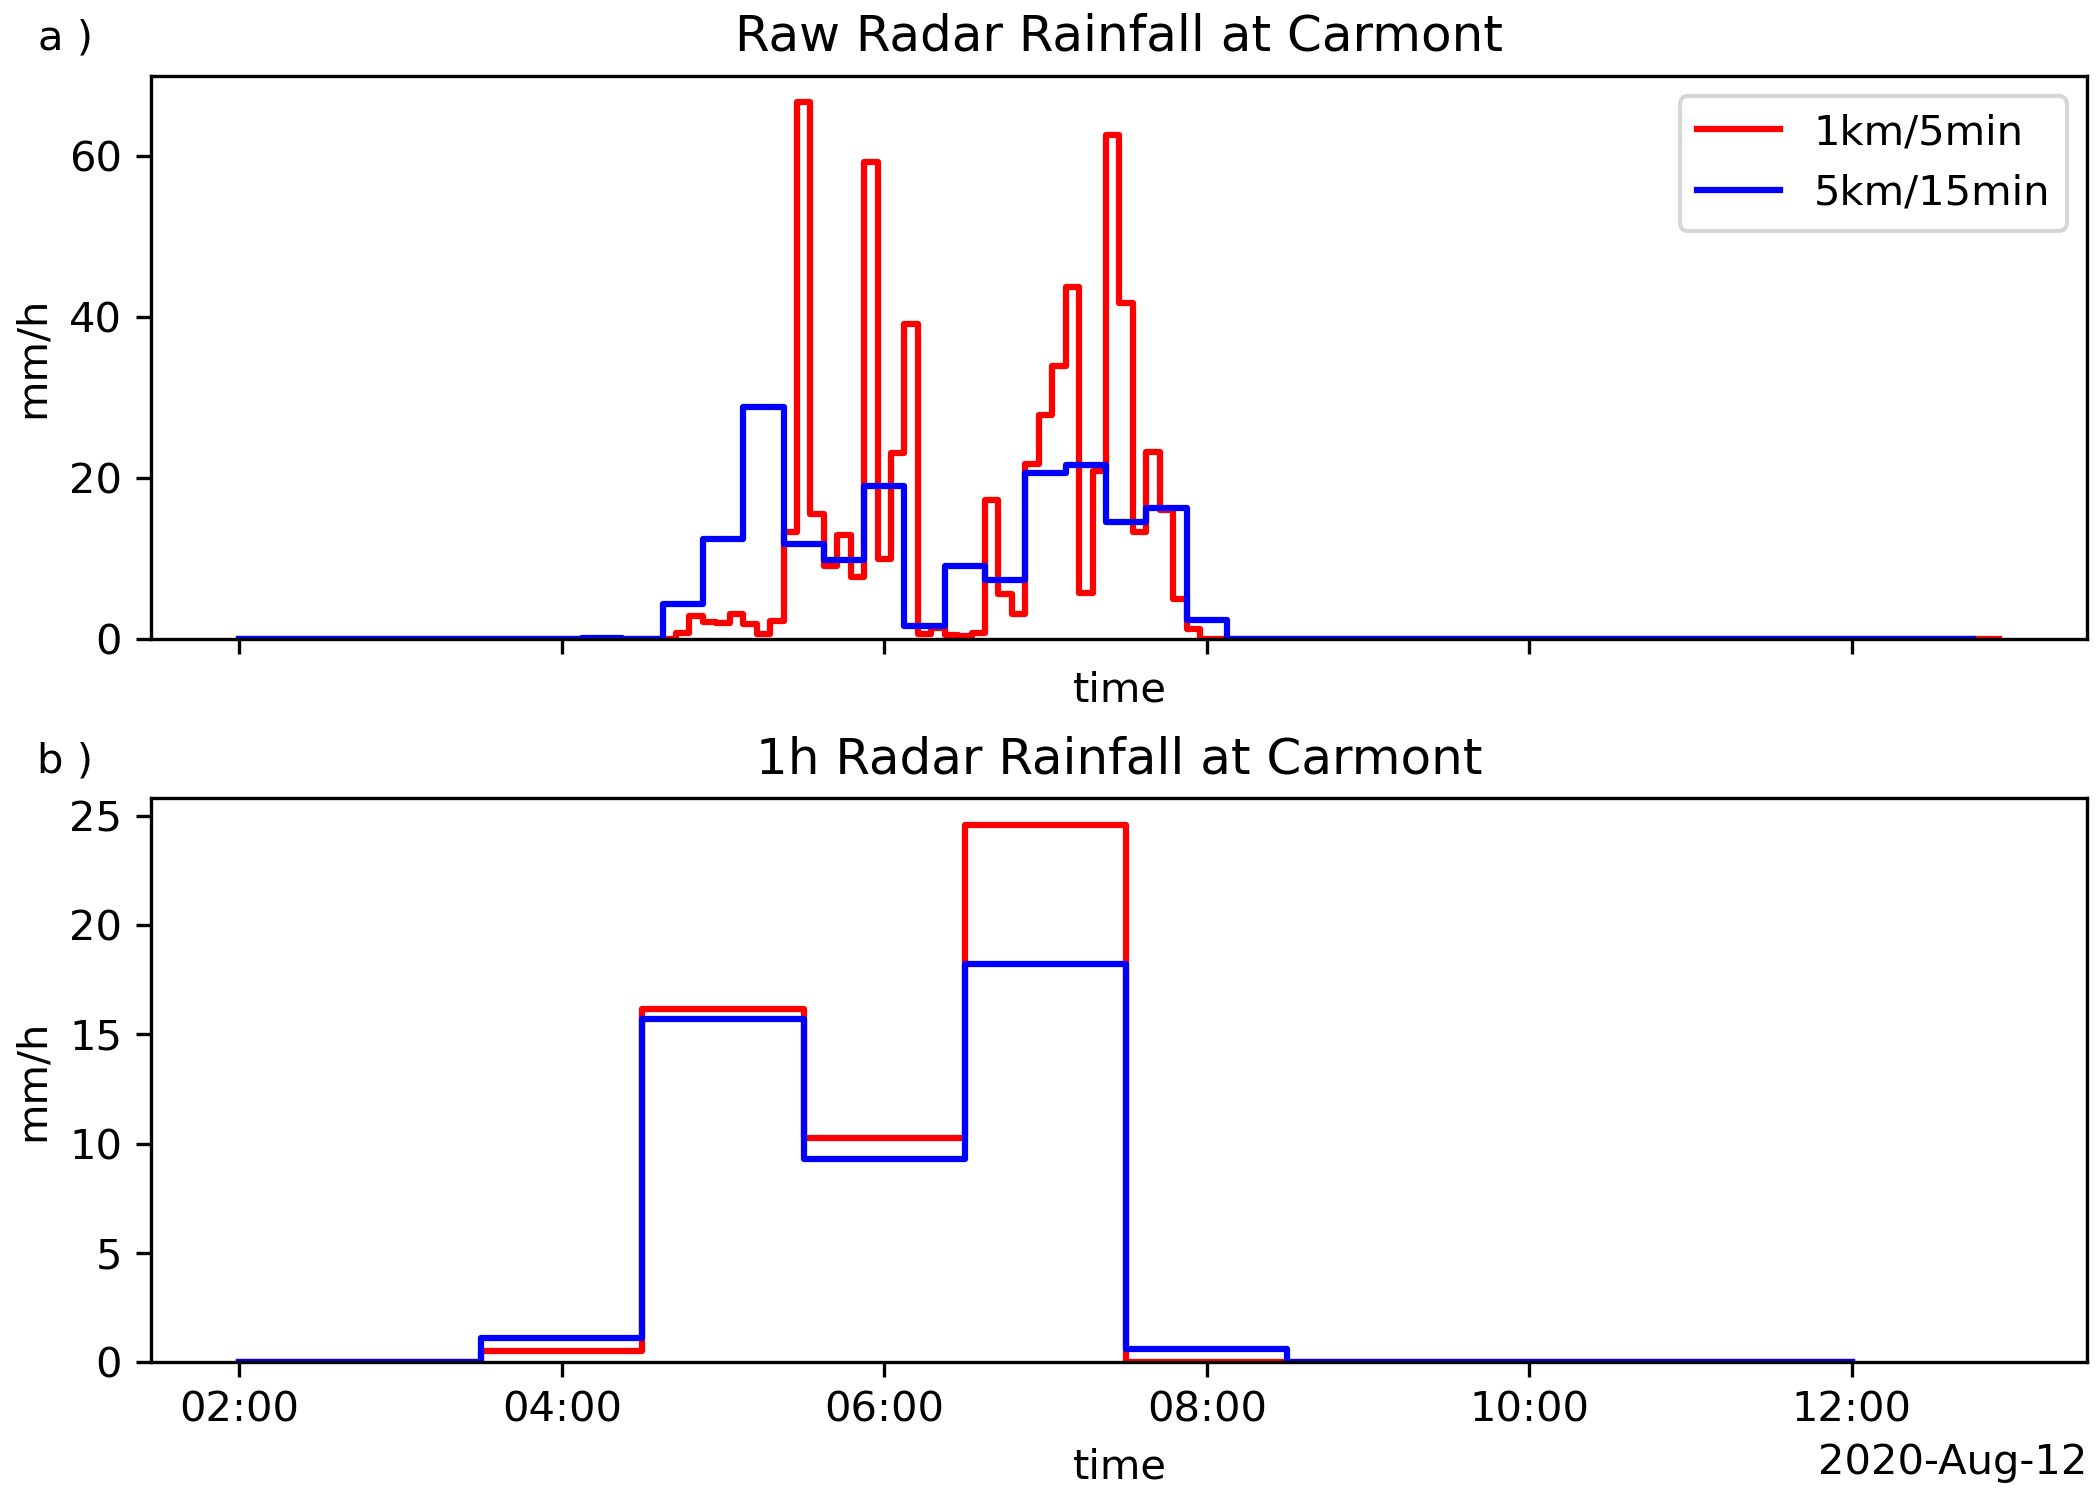
\includegraphics[width=0.5\linewidth]{radar_carmont.png}
	\caption{a) Radar rainfall rates at Carmont (mm/h) for 1km/5 min (red) and 5km/15 min; b) Hourly mean rates for 1km (red) and 5km (blue) radar data. Data is shown from 2020-08-12T02:45 to 10:15. }
	\label{fig:mean_rain}
\end{figure}

\begin{figure}[tp]
	
	\centering
	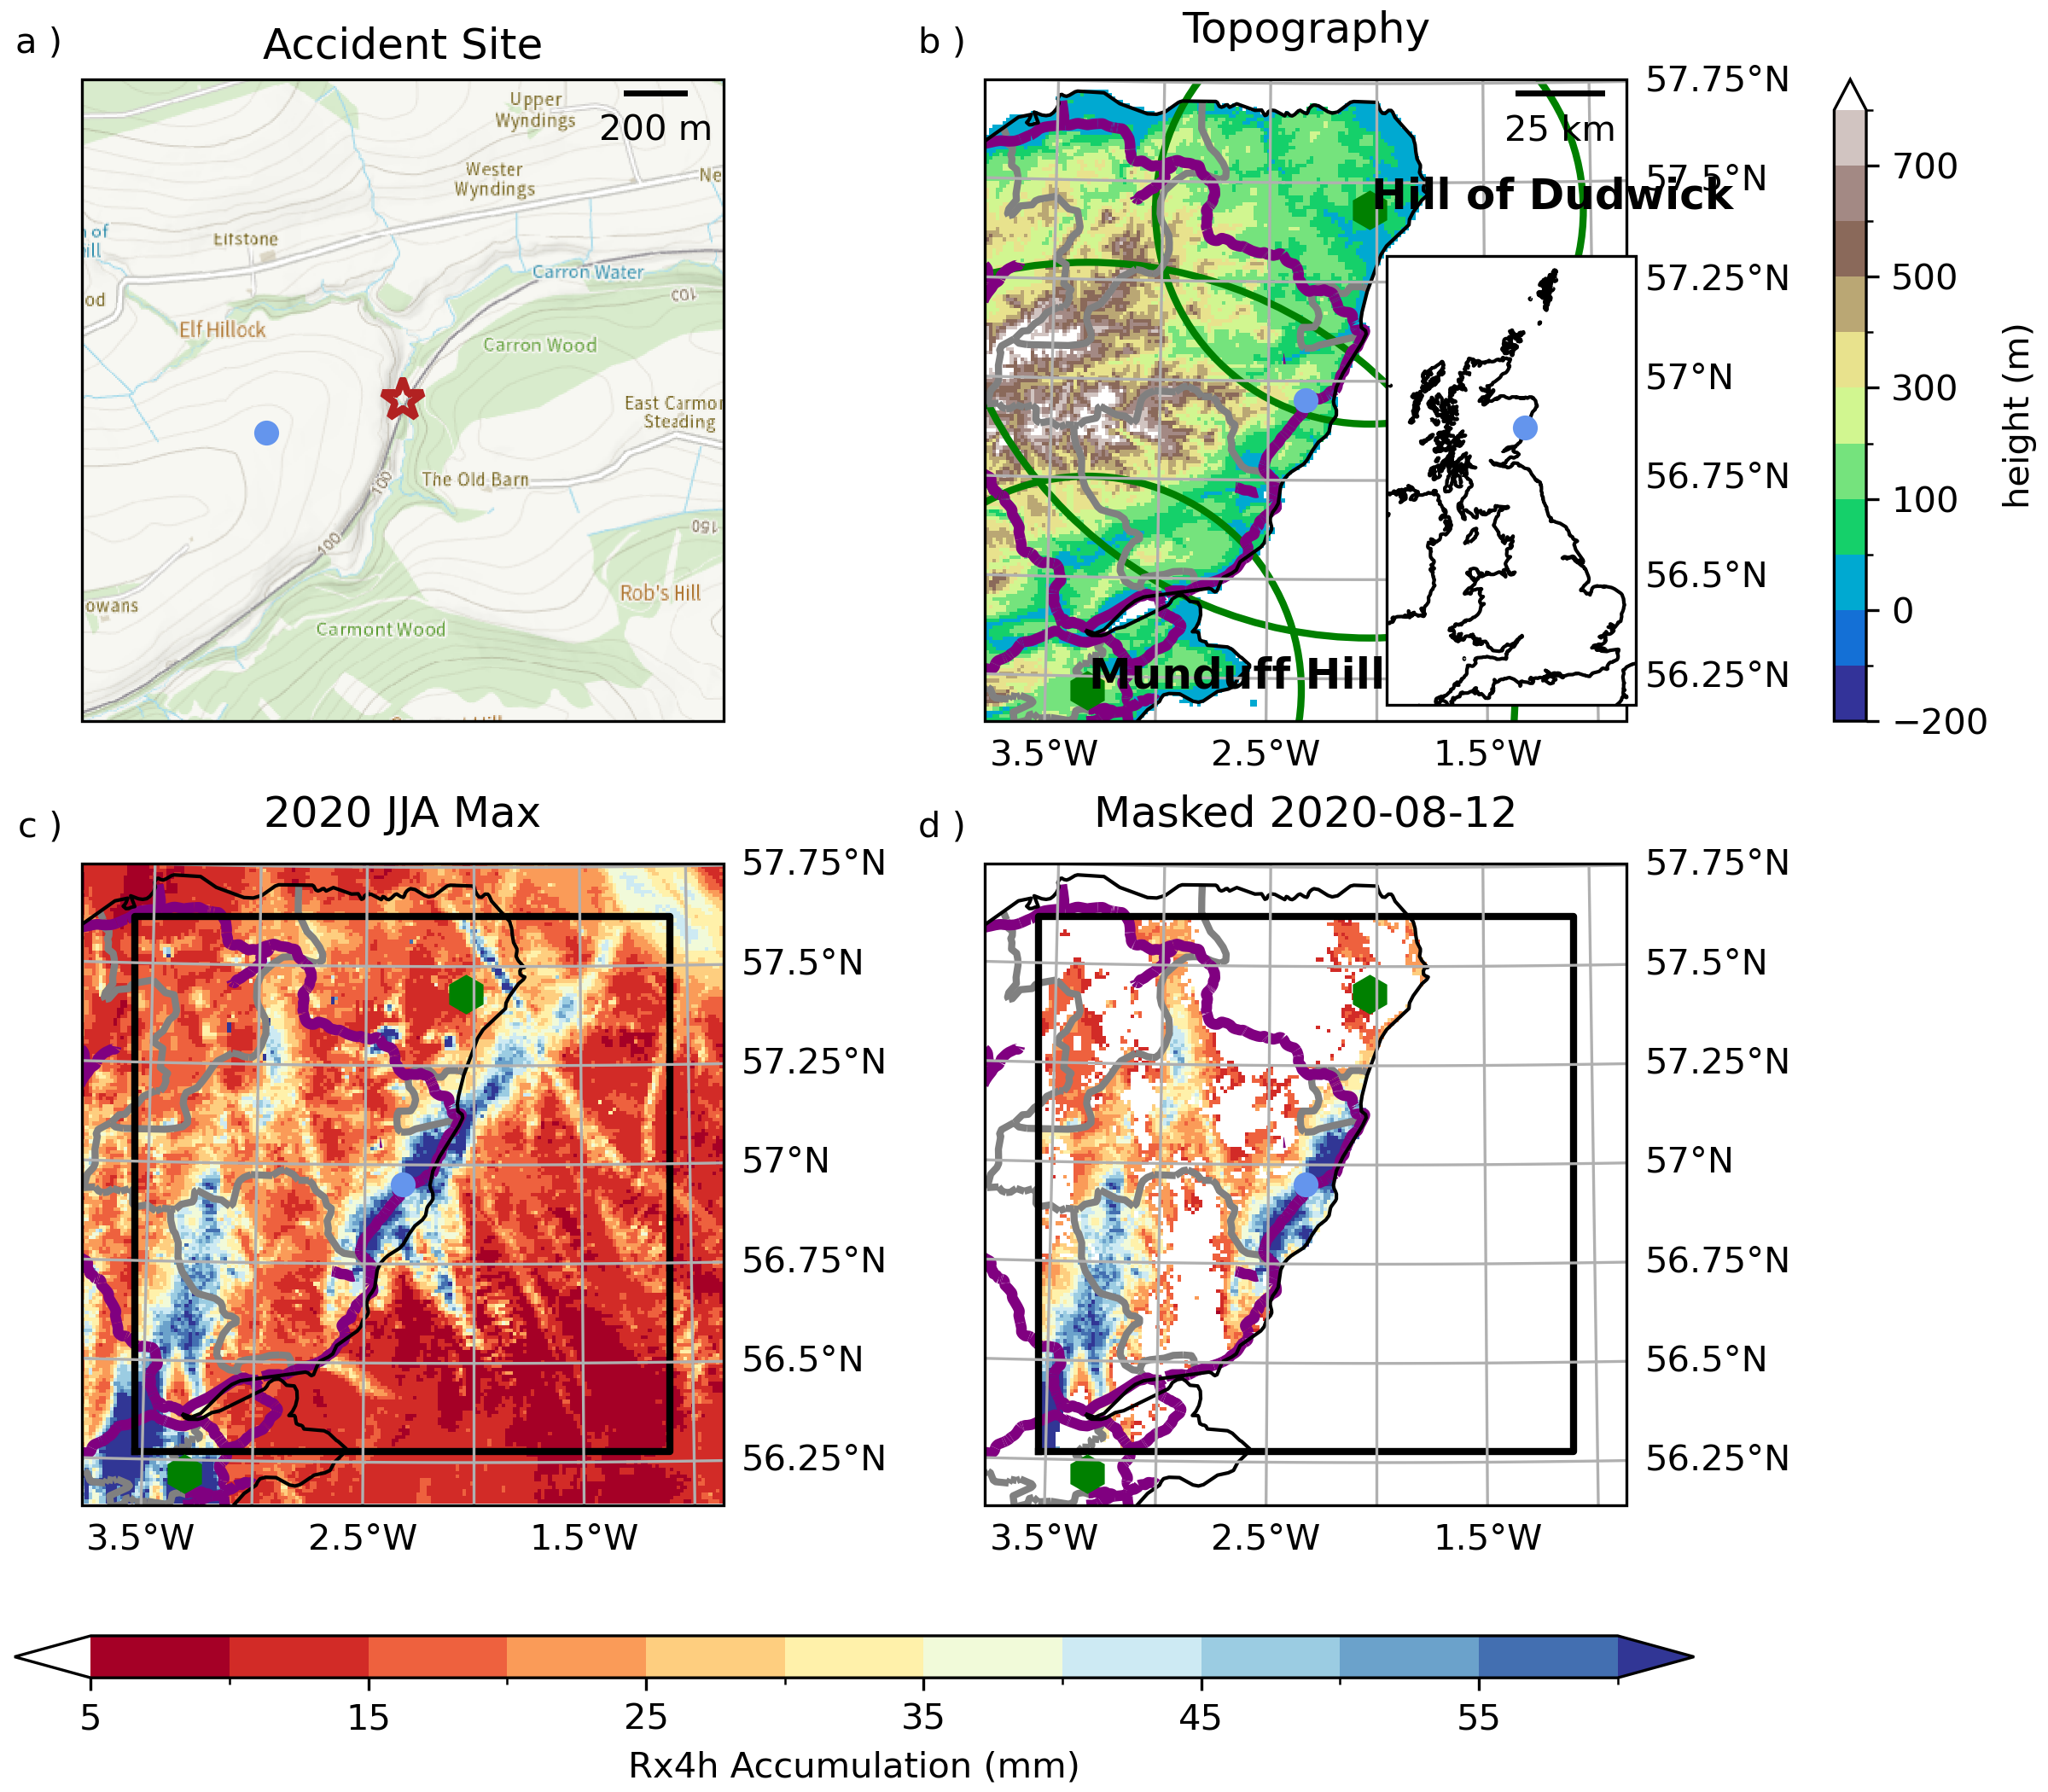
\includegraphics[width=\linewidth]{carmont_geog_group.png}
	\caption{a) Map of Carmont Accident site -- brickred star shows where train derailed. Main features are contour lines every 10 meters, railway (black line ) and woods (green) (Map crown copyright Ordinance Survey). b) Topography of North East Scotland. Inset shows Great Britain and Ireland. Colour scale on bar to right. Circles are  60 and 120 km from radar stations.  c) Maximum 4 hour accumulation  for JJA 2020. d) Event of 2020-8-21.  Black box in c \& d shows 150x150 km region of interest. Scale bars are shown in a and b.   }
	\label{fig:carmont_geog_group}
\end{figure}





\begin{figure}[tp]
	\centering
	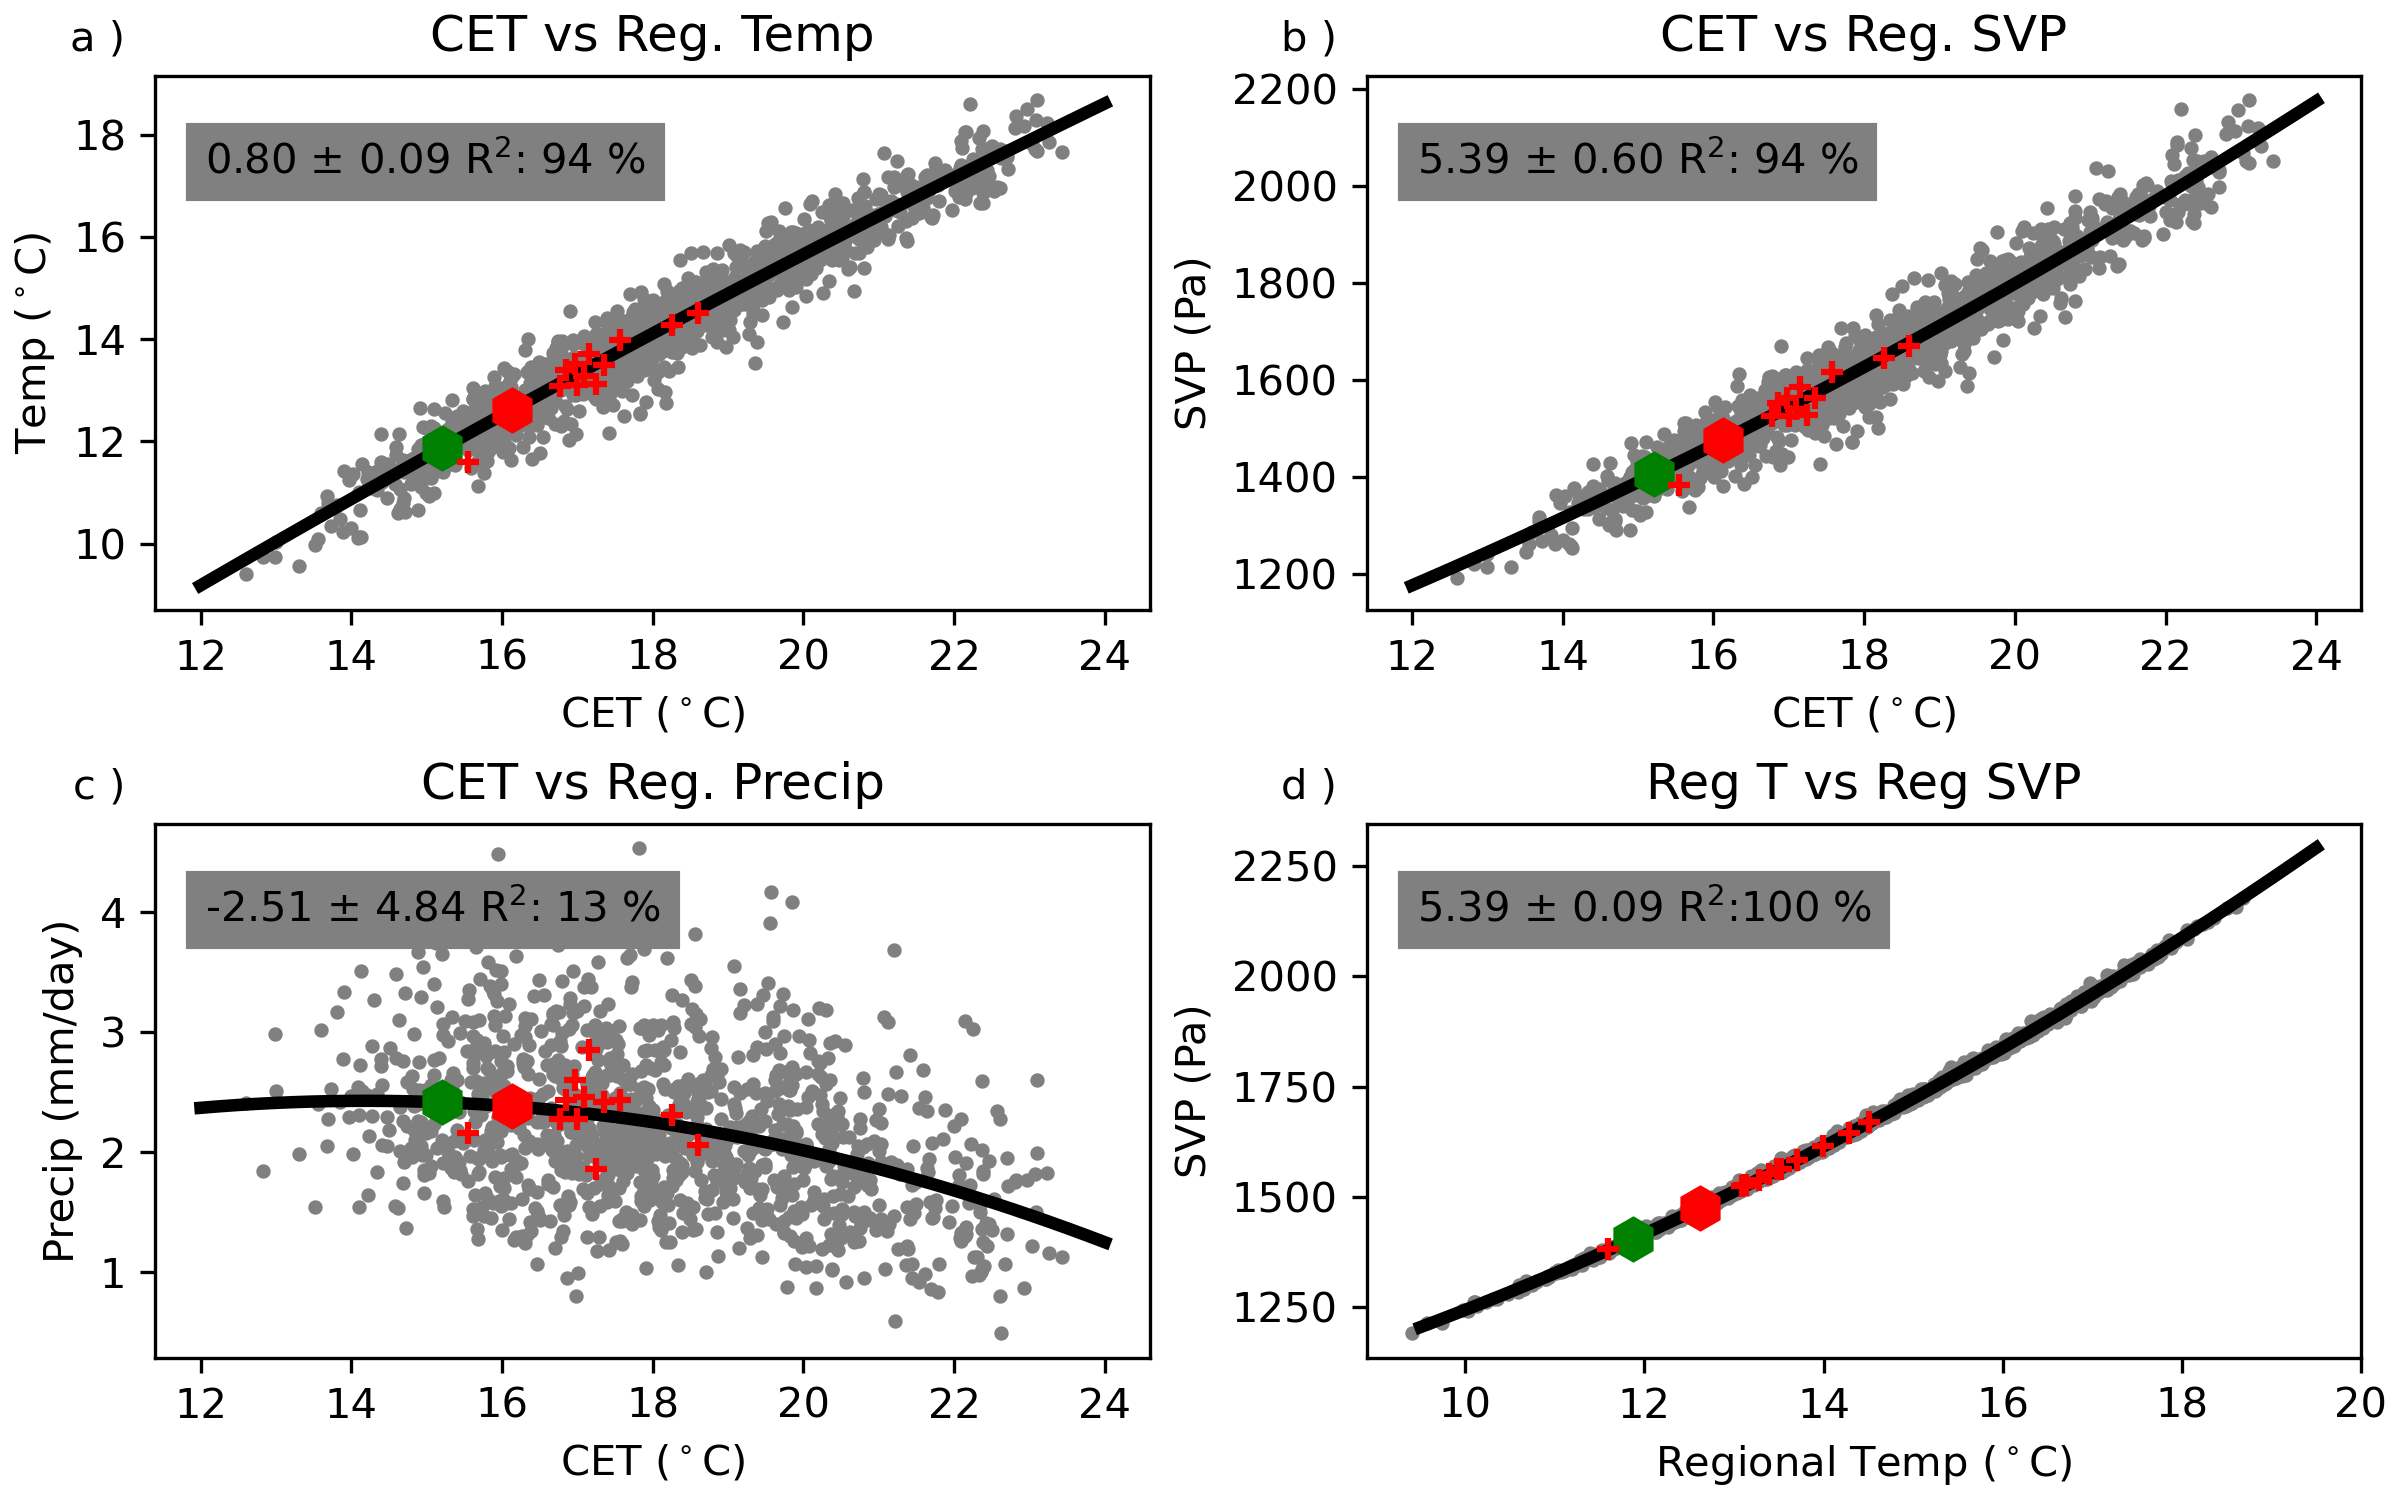
\includegraphics[width=\linewidth]{scatter.png}
	\caption{Scatter plots for summer mean  a)  Central England Temperature (CET) vs  regional mean temperature; b) CET vs regional average saturated vapour pressure (SVP); c) CET vs regional average precipitation; d) Regional temperature vs Regional SVP. Green and red hexagons show estimated 1850-1899 and 2012-2021 average values. Lines show second order best fits.}
	\label{fig:cet_scatter}
\end{figure}



\begin{figure}
	\centering
	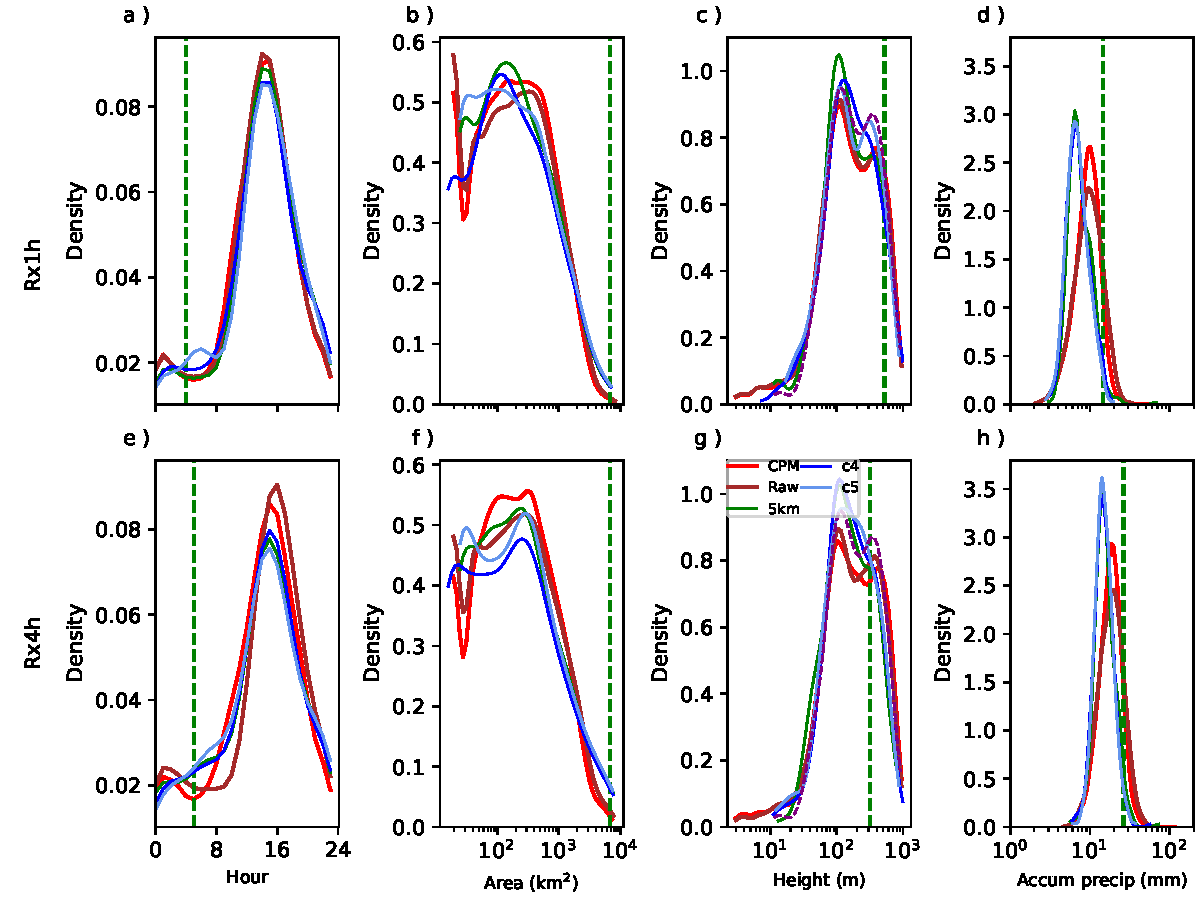
\includegraphics[width=\linewidth]{kde_smooth_events}
	\caption{Kernel Density Estimates from  CPM (orange), 5km radar (green), 1km-c4 (blue) and 1km-c5 (pale blue) events at 50\% quantile for 2008-2022 period. Shown are day-hour (a \& e),$\log_{10}$ of event area (b \& f),  topographic height (c \& g ) and maximum Rainfall accumulation (d \& h). Top row shows Rx1h while bottom row shows Rx4h values.}
	\end{figure}




    
%    \begin{figure}
%    	\centering
%    	\includegraphics[width=\linewidth]{fit_ratio.png}
%    	\caption{a) \% change per degree CET change in location parameter between 2061-2080  and 1981-2000 for all events in the filtered UKCP ensemble. b) as a) but for scale parameter. c) Shape parameter for 1981-2000 (blue) and 2061-2018 (orange) data. All results are shown as a function of event quantile and errors bars are $\pm2\sigma$. Dotted lines in a) \& b) show mean value of the parameter. Dashed horizontal line in c shows shape value of 0.}
%    \end{figure}
\begin{figure}
\centering
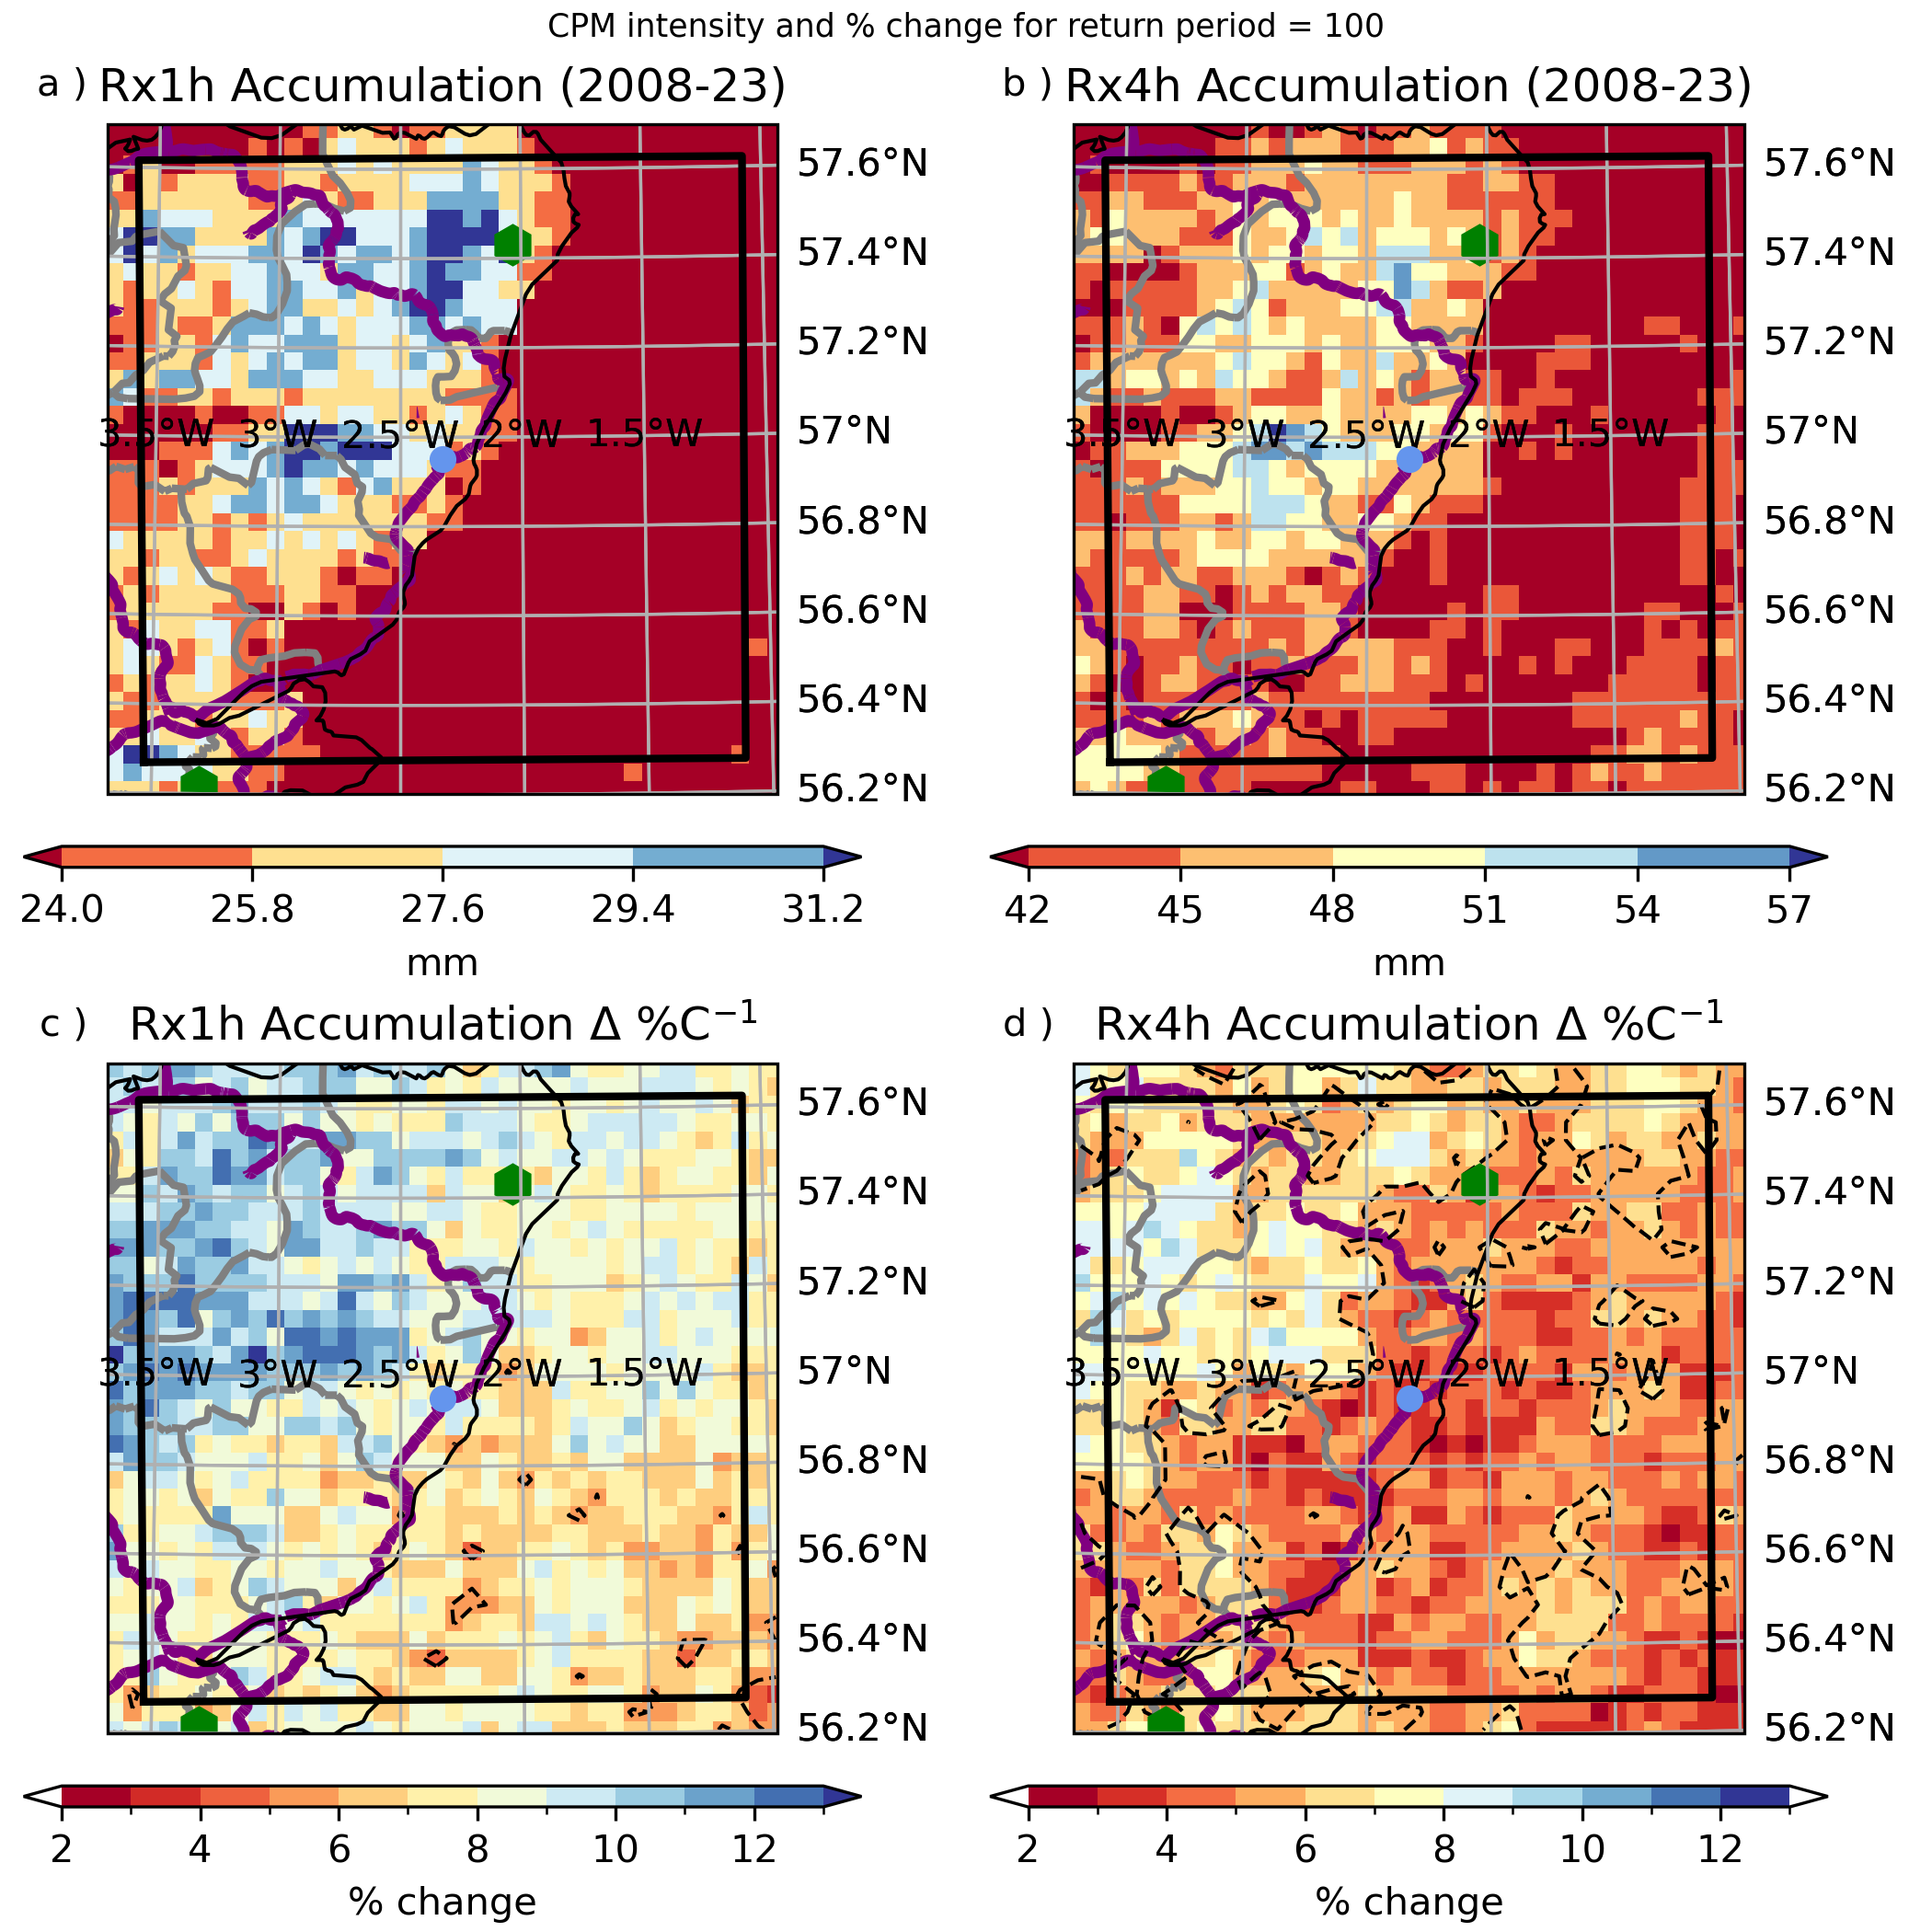
\includegraphics[width=1\linewidth]{cpm_intensity_delta}
\caption{One in a hundred year CPM maximum rainfall accumulation for 1 and 4 hour rainfall (a \& c) and percentage sensitivity to 1 degree CET increase. Dashed lines shows intensity increase of 5.5\%/degree CET corresponding to CC. Other elements as Figure~\ref{fig:carmont_geog_group}  }
\label{fig:map_intensity}
\end{figure}

\begin{figure}
	\centering
	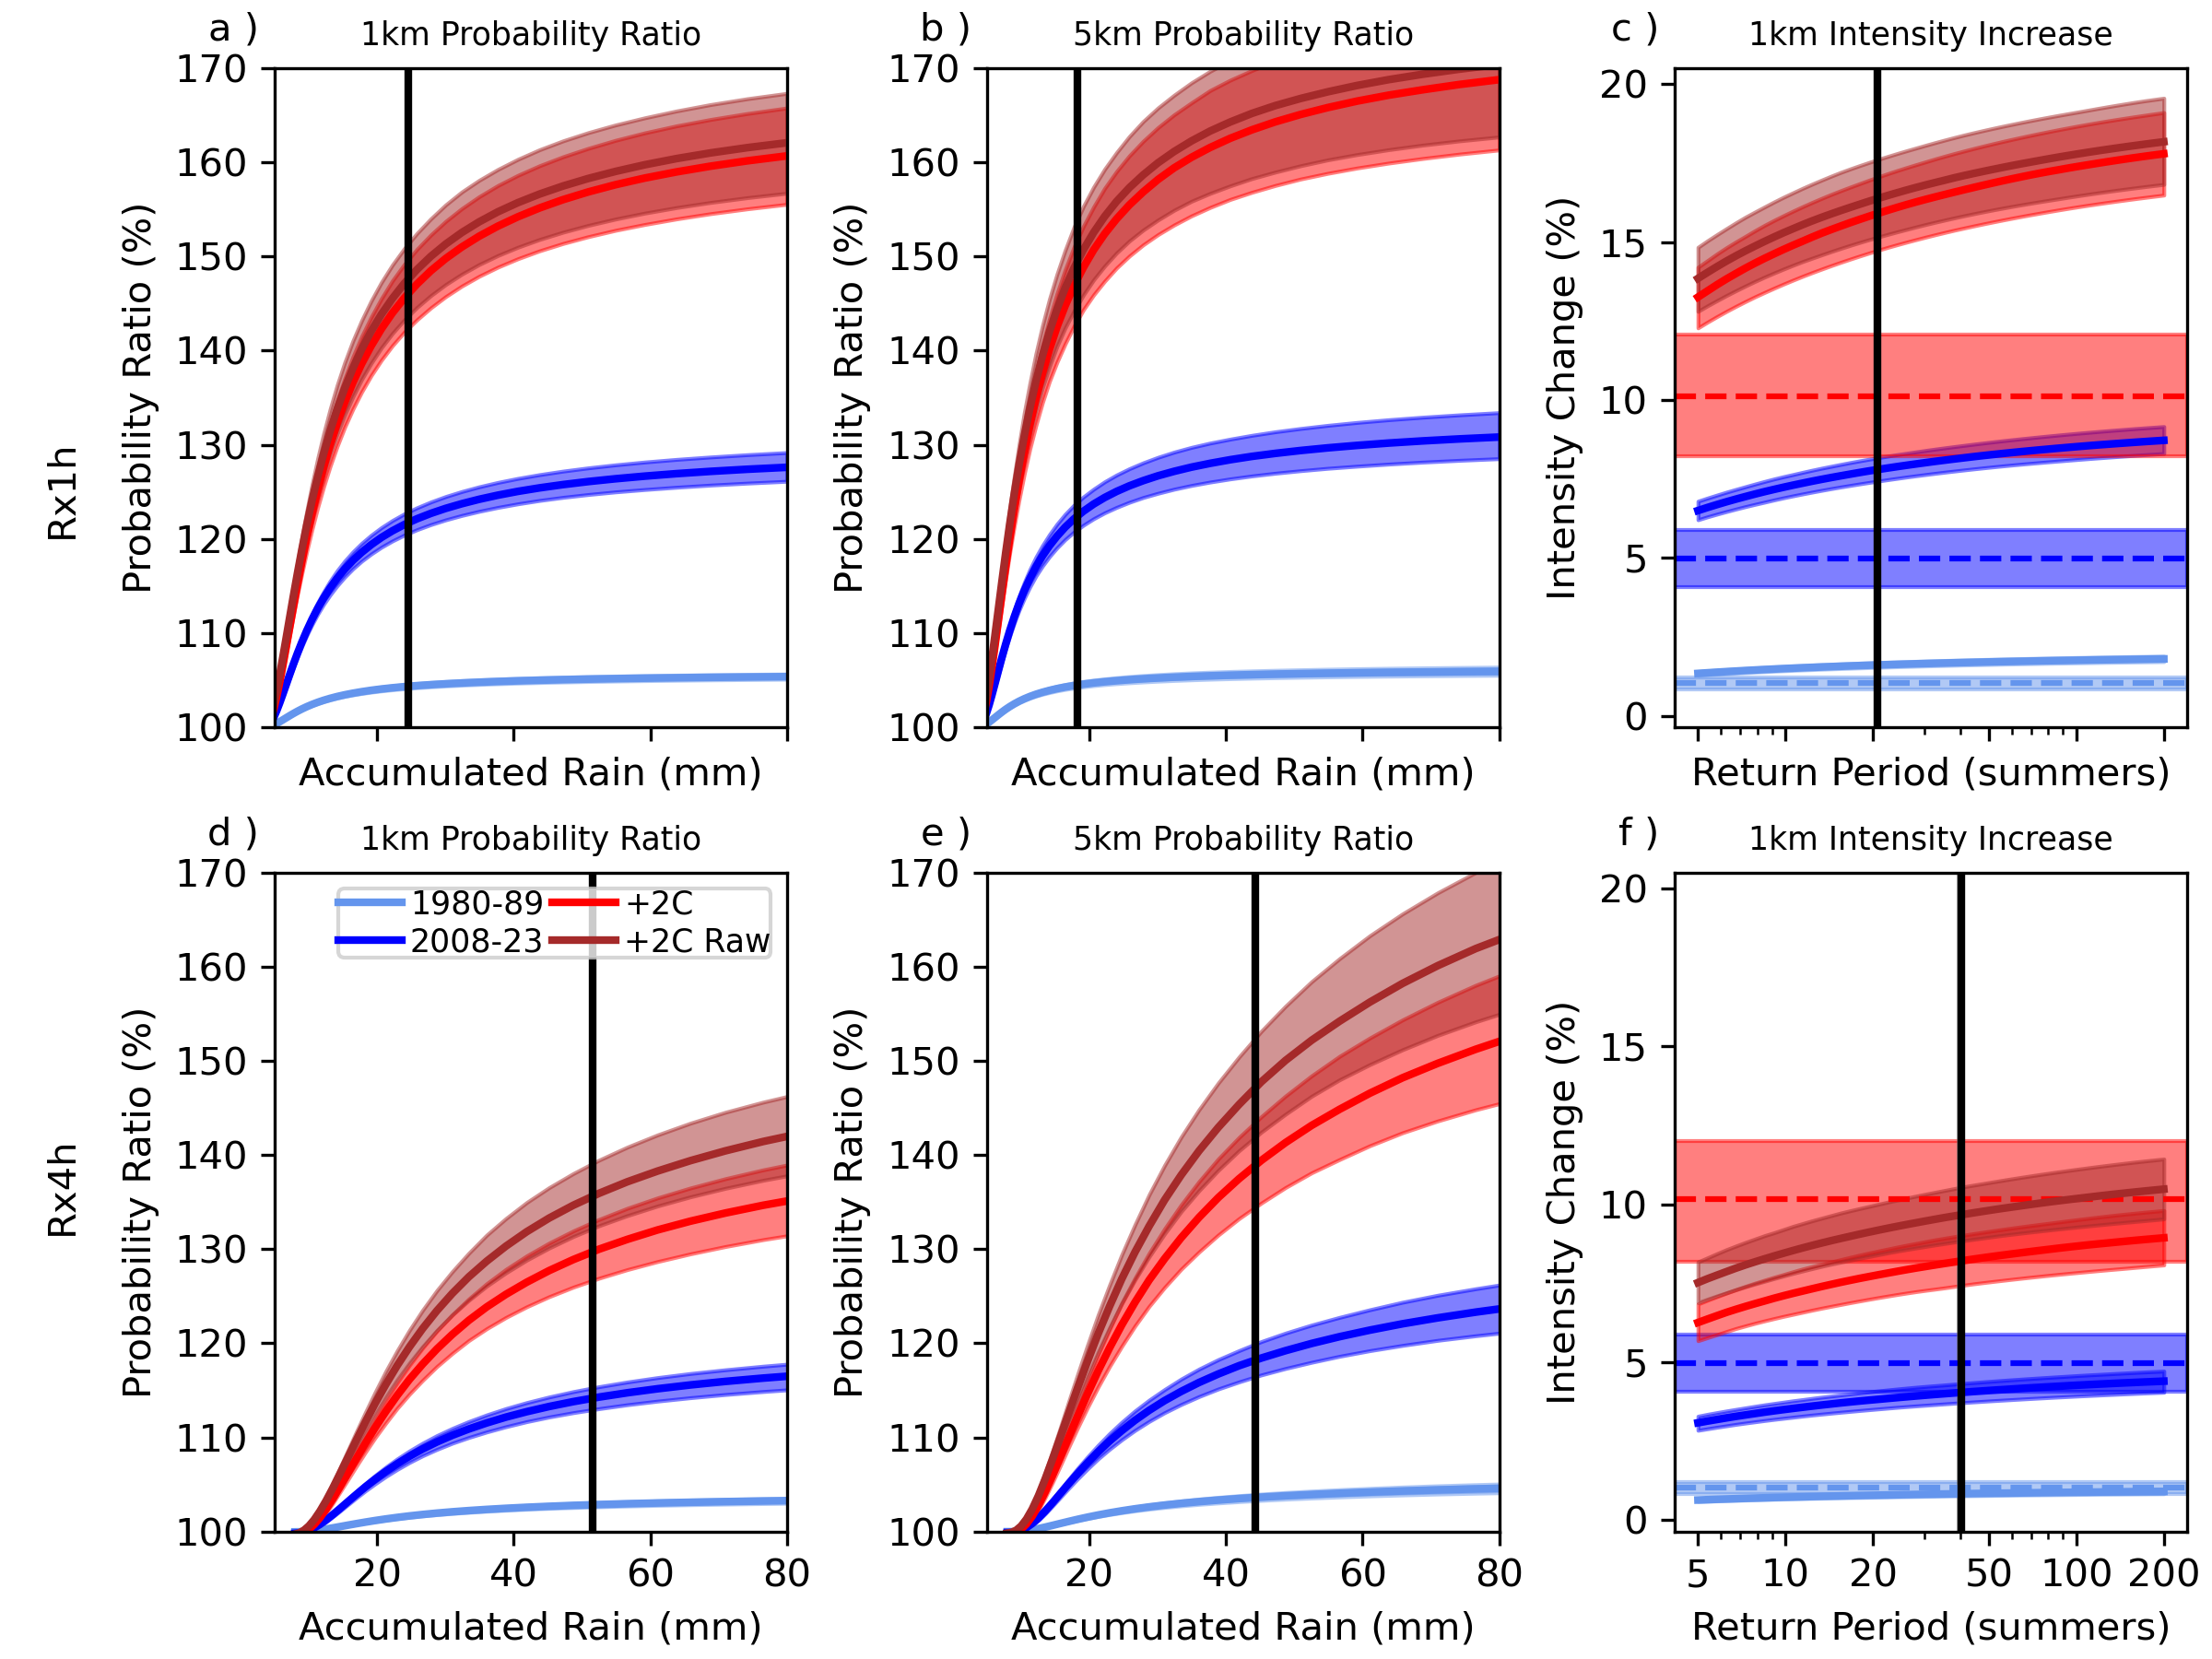
\includegraphics[width=1\linewidth]{intens_prob_ratios}
	\caption{a: Changes in filtered CPM Rx1h intensity (\% of PI values) as function of return period. b) Probability ratio (\%) relative to Pre-industrial as a function of summer seasonal Rx1h. Shown are changes for +2K world (red), 2012-2021 (dark blue) and 1980-1989 (pale blue). Also shown are 5-95\% range from regional fits (shaded regions) and median regional intensity change and probability ratios (dot-dashed lines).}
	\label{fig:int_pr}
\end{figure}



\end{document}
